\def\Module{Principles of Computer System Design}
\def\Uebung{Assignment 1}
\def\Studentenname{Marcus Voss (qcz284), Robert Schmidtke (rxt809), Marco Eilers (dbk726)}
\def\Sub_date{06.12.2012}

\documentclass[12pt,a4paper]{article}

\usepackage[utf8]{inputenc}
\usepackage[T1]{fontenc}
\usepackage{fullpage} 
\headsep1cm
\parindent0cm
\usepackage{amssymb, amstext, amsmath}
\usepackage{fancyhdr}
\usepackage{lastpage}
\usepackage{booktabs}
\usepackage{graphicx}
\usepackage{subfigure}
\usepackage{hyperref}
\usepackage{threeparttable}
\usepackage{footnote}
\usepackage{listings}
\makesavenoteenv{tabular}

\lhead{\textbf{\Module}}
\rhead{\Uebung~(Submission: \Sub_date)}

\cfoot{}
\lfoot{\Studentenname}
\rfoot{\thepage\ of \pageref{LastPage}}
\pagestyle{fancy}
\renewcommand{\footrulewidth}{0.4pt}

\newcommand{\code}[1]{{\fontfamily{fvm}\small \selectfont #1}}

%Line spacing between paragraphs
\setlength{\parskip}{6pt}

\begin{document}

\title{\Module\\\Uebung}
\author{\Studentenname}
\maketitle

\section*{Exercises} 
\label{sec:exercises}

\subsection*{Question 1}
\label{sec:eq1}
\subsubsection*{(a)}
Our abstraction would have one central component which receives all read/write requests from the clients and translates them into one or several requests (if the area that should be read or written to is distributed over several machines) for the individual machines, waits for the result, combines the results if necessary and sends it back to the clients. All information concerning the abstraction would be kept in this component; neither the clients nor the individual machines have to know that there is any abstraction at all. We could translate addresses by assigning an offset to each of the storage machines: the first machine would have the offset zero, and the $n$th machine would have the offset $offset(n-1) + storageSize(n-1)$. Computing the ID of the machine and the physical memory address from an address in the global address space would then mean finding the two offsets between which the address lies and subtracting the lower offset from it.
We do not actually have many other choices for the translation of storage addresses, since we need to provide a continuous address space.
However, the translation can be simplified if all storage machines provide the same amount of storage and the size of this storage is a power of two; in this case the first few bits of the global address will be the ID of the machine, and the following bits denote the physical address, so that only two simple bitwise operations are necessary.

The central component would also have to regularly check if all machines are still online, and inform clients when their requests cannot be fulfilled because a machine needed for their completion cannot be reached. 

In this scenario, all traffic has to pass the central component for every transaction, so this component is an obvious bottleneck. It would therefore be a good idea to have several instances of this central component. Each could work on its own, so there are no synchronization issues. A load balancer could be used to make sure that all such components are used equally. In this case, the storage should scale very well since more manager components can be added at will. With only one such component, however, the whole storage's performance is would be limited by the central component and would not scale at all after this point.
\subsubsection*{(b)}
\begin{itemize}
  \item \texttt{getStorageAttributes()} would tell the clients basic information about the memory, like size and the current status (e.g. online, offline, storage server down). It would take no arguments and return a data structure containing the information.
  
  \begin{lstlisting}[basicstyle=\footnotesize]
  getStorageAttributes(){
      return {Size: this.size,
              Status : this.status};
  }
  \end{lstlisting}
  \item \texttt{read(long address, int length)} takes the address from which the client wants to read and the length of the segment that should be read in bytes. It returns an array of bytes of the specified length if everything succeeds, otherwise it returns an exception.
  \begin{lstlisting}[basicstyle=\footnotesize]
  read(long address, int length){
      if (address + length > STORAGE_SIZE)
          throw new InvalidArgumentException();
  
      // find the correct storage machine
      Long offset;
      Integer segmentLength;
      Long nextOffset;
      Integer machineID;
      
      for (i = 0; i < servers.length; i++) {
          if (address >= servers[i].getOffset()
              && address <= servers[i+1].getOffset()){
              offset = servers[i].getOffset();
              segmentLength = servers[i].getLength();
              nextOffset = servers[i+1].getOffset();
              machineID = servers[i].getMachineID();
              break;
          }
      }
      
      // read data from storage
      Address serverAddress = mappings.get(machineID);
      
      // check if segment reaches into next machine's space
      Long end = address + length;
      Long overlap = end - nextOffset;
      Int readLength = length;
      
      if (overlap > 0)
          readLength -= overlap;
      
      sendReadRequest(serverAddress, length);
      
      response = waitForResponse (TIMEOUT);
      if (response == null)
          trow new TimeoutException();
      if (response.success){
          if (overlap < 0)
              return concat (response.getData(),
                            read(nextOffset, overlap));
          else
              return response.getData();
      }else{
          throw response.getException();
      }
  }
  \end{lstlisting}
  
  For the simplified translation method where all storage machines have the same capacity, the address translation could look like this:
  \begin{lstlisting}[basicstyle=\footnotesize]
  read(long address, int length){ 
      ...
      // find the correct storage machine     
      Integer machineID = address / SERVER_CAPACITY;
      Address serverAddress = mappings.get(machineID);
      
      Long nextOffset = (machineID+1) * SERVER_CAPACITY;
      
      // read data from storage
      ...
  }
  \end{lstlisting}
  
  \item \texttt{write(long address, byte[] data)} takes the address that should be written to and the data that should be written. It would not return anything unless a problem occurs, in which case it would throw an appropriate exception. Since the translation of addresses is the same as in read, we will only include the simplified version here.
  
  \begin{lstlisting}[basicstyle=\footnotesize]
  write(long address, byte[] data){
      Integer length = data.length;
      if (address + length > STORAGE_SIZE)
          throw new InvalidArgumentException();
          
      // find the correct storage machine     
      Integer machineID = address / SERVER_CAPACITY;
      Address serverAddress = mappings.get(machineID);
      
      Long nextOffset = (machineID+1) * SERVER_CAPACITY;
      
      // write data to storage
      Address serverAddress = mappings.get(machineID);
      
      // check if segment reaches into next machine's space
      Long end = address + length;
      Long overlap = end - nextOffset;
      Int writeLength = length;
      byte[] writeData = data;
      
      if (overlap > 0){
          writeLength -= overlap;
          writeData = data.subArray(0, writeLength);
      }
      
      sendWriteRequest(serverAddress, writeData);
      
      response = waitForResponse (TIMEOUT);
      if (response == null)
          trow new TimeoutException();
      if (response.success){
          if (overlap < 0)
              write (nextOffset, data.subArray(writeLength, length));
      }else{
          throw response.getException();
      }
  }
  \end{lstlisting}
\end{itemize}


\subsubsection*{(c)}
We would definitely make basic operations non-atomic (unless we know for certain that our memory abstraction will only ever be used for purposes that always require atomicity). Guaranteeing atomicity always comes with a performance cost, and a basic component like memory should offer the possibility to read and write as fast as possible for cases where atomicity is not needed. It is always possible to make wrappers for existing functions that do guarantee atomicity, whereas it is not possible to get rid of the overhead if atomicity is implemented in the memory (abstraction) itself. If one wanted to create atomic functions on top of the provided ones, one could simply create read-write-locks for every unit of memory (e.g. for every page) and lock or unlock those before and after every read or write.

\subsection*{Question 2}
\label{sec:eq2}

\subsubsection*{(a)}
\begin{table}[htbp]
\caption{Comparison of Storage}
\begin{center}
\begin{tabular}{|p{0.35\textwidth}|p{0.18\textwidth}|p{0.18\textwidth}|p{0.18\textwidth}|}
\hline
 & Hard disk & SSD & Main Memory \\ \hline
1 Access time read/write & 6.78 ms/8.83 ms & 0.04 ms/0.05 ms & 100 ns/100 ns \\ \hline
2 Average Capacity & 1 TB & 128GB & 16GB \\ \hline
3 Cost per unit & 267.59\$ ($\frac{0.26\$}{GB}$) & 109.99\$ ($\frac{0.86\$}{GB}$) & 390.00\$ ($\frac{24.37\$}{GB}$) \\ \hline
4 Reliability (MTBF, volatility) & 1-1.5 mio. hours, non-volatile & 1-2 mio. hours, non-volatile & 6-11 mio. hours, versatile \\ \hline
5 Power Consumption idle/typical/max write (per h) & 4/6.5/5.5 watt& 0.3/1.3/2.5 watt & about 4 watt \\ \hline
\end{tabular}
\end{center}
\label{tab:storage}
\end{table}

Table \ref{tab:storage} shows evaluation numbers obtained from a web search. For hard disk (HDD) and solid state disk (SSD) the numbers for dimensions 1-3 and 5 are well comparable as they are from the same source. Numbers where taken from the fastest (access reading time) hard disk\footnote{\url{http://www.tomshardware.com/charts/hdd-charts-2012/compare,2898.html?prod\%5B5531\%5D=on} [last accessed: 03.12.2012]} and SSD\footnote{\url{http://www.tomshardware.com/charts/ssd-charts-2012/compare,2788.html?prod\%5B5837\%5D=on} [last accessed: 03.12.2012]} in the respective benchmark test for each of the categories\footnote{\emph{HDD Charts 2012} and \emph{SSD Charts 2012}}. These numbers are however for desktop systems, but we can assume that it is in the same range for server systems. To assess reliability in terms of media failure, a common measure is Mean Time Before Failure (MTBF, but also found as Mean Time To Failure). The figures for the HDD is from \cite{Schroeder2007} and gives a range that is typically stated to be 1-1.5 mio. hours\footnote{Although the paper analyses these claims and finds that these numbers are mostly exaggerated}. For SSD we could find a similar range of about 1-2 mio. hours\footnote{\url{http://solid-state-drive-review.toptenreviews.com/} [last accessed: 03.12.2012]}. For reliability we want to further distinguish between volatility and non-volatility, as in the case of a crash the data in RAM is generally lost, while it is still there in HDD and SSD. Finding specific and reliable numbers for main memory (RAM) was not as easy as for the storage disks, as they are benchmarked in different ways and with different measures. Access times are not found that specifically. However, they are in a much smaller range. While disk access times (SSD and HDD) are reported in milliseconds ($10^{-3}$), they are in the range of nanoseconds for RAM ($10^{-9}$), as found in \cite{Dean}. Figures for reliability and power consumption where not found from reliable sources, and are only estimates based on posts in forums\footnote{MTBF: \url{http://www.theriac.org/forum/showthread.php?t=12954} and power consumption: \url{http://answers.yahoo.com/question/index?qid=20100711051719AAVSIhe},
\url{http://www.tomshardware.com/reviews/lovo-ddr3-power,2650.html} [all last accessed: 03.12.2012]}. Also the size and price ranges depend a lot on the type of system. We chose rather randomly a representative example\footnote{\url{http://h30094.www3.hp.com/product.aspx?sku=10239599} [last accessed: 03.12.2012]}.

\subsubsection*{(b)}

As shown in \emph{a)} the speed of RAM still a lot faster than the disk based memories - even when compared to the already fast SSD (e.g. about 400 times faster for our numbers). However, the cost per GB is much higher for RAM when compared to the disk based memories (with our numbers almost 100 times more expensive than HDD, and almost 30 times more than SSD). So when designing a distributed memory abstraction such as above, a first trade off is between price of storage and speed. The HDD is currently the cheapest memory, but very slow, when compared to SDD, and especially RAM. But the SSD could certainly become an alternative to consider, especially as its costs are currently decreasing, and the common disk sizes are increasing, so that the gap to HDD in regard to these dimension becomes smaller and smaller - with a vast improvement in the speed dimension. In terms of reliability there were no significant differences in terms of failures, but the disk based memories are non-volatile! So deploying e.g. SSDs as part of the above system could increase overall reliability of the system if crucial parts, such as logs for recovery, are stored on SSD. In the dimension of power consumption we could also find no significant differences between these technologies. Here other parts of the system such as the CPU are rather worth investing in to lower power consumption.

\subsection*{Question 3}
\label{sec:eq3}

\subsubsection*{(a)}
While concurrency usually has a positive effect on a system's latency, there may also be cases where this effect is only marginal or even negative. In general, the ability to process several requests at once means that some requests can be worked on right away instead of having to wait for the completion of another request, or at least that waiting time is reduced. However, this is only true if the system's utilization is high enough. If, on the other hand, the system's utilization is low and it only ever has one request at a time do work with, concurrency will not have a positive effect at all. In this case, it might even have a slightly negative effect, since the added overhead for work distribution and scheduling will add to the latency of every single request.

In the above paragraph, we assumed that the system's hardware natively supports concurrency, which is usually the case nowadays, so that several units of work can actually be executed at the same time. If, however, the system only simulates concurrent execution, the impact on the latency will quite probably always be negative. In this case the system would start working on several tasks at once and distribute the processor's computing time between them. While fewer (or no) tasks would have to wait before they are started, the work on every task will take considerably longer. Combined with the overhead from scheduling etc., the overall latency would be at least as high as with serial execution.

\subsubsection*{(b)}
Batching means performing a number of related tasks at the same time instead of doing each one on its own, usually in order to reduce the overall overhead: Often the overhead for specific tasks stays the same, independent of the size of the task. In this case it can be advantageous to combine several tasks into one, so that the overhead occurs only once and not once for every task. There may be additional performance benefits that arise from similarities or a certain order of the tasks. 

Dallying, on the other hand, means that one delays the execution of a task to get some kind of performance benefit. One reason to do this is because it might not actually be necessary to execute the task after all (but this is not yet clear). The other reason is related to batching: One delays the execution of several small tasks and waits until a certain number of such tasks has been collected. This collection of tasks is then executed at once (using batch execution) in order to profit from the reduced overhead, as described above. Batching may therefore be a part of (or a motivation for) dallying.

Both batching and dallying are quite common in computing as well as in the real world. Message passing is an example where batching can reduce the overall overhead considerably, since the static overhead for sending one large message is usually much lower than for sending several smaller ones. An example where dallying could be used is our key-value-store: if there are several operations on a single key, one of which negates the effects of a previous one (e.g. overwrote or deletes the value), then the operation(s) before the last operation can be left out. A real world example where dallying is used to use batching is washing dishes: If one waits for a few days until washing dishes again, one can wash more plates at once, and therefore the overhead of letting water into the sink etc. occurs only once instead of several times.

\subsubsection*{(c)}
Caching is a perfect example for fast path optimization. It means that, in addition to the normal and relatively slow way of accessing data, which usually means accessing RAM or a disk or network resource, there is another, much faster way for common requests. This faster way does not work for all kinds of requests (otherwise one would not use the slower one at all), in our case because a cache is typically at least an order of magnitude smaller than the actual memory. A good cache therefore contains those parts of the memory that are accessed most frequently, and getting data from the cache is much faster than getting them from the actual memory. 

\subsection*{Question 4}
\label{sec:eq4}

\subsubsection*{(a)}
Typical caches use two properties to decide which parts of the memory to keep in the cache: temporal locality and spatial locality. This means that data is cached if a) it has been requested in the (recent) past or b) it is physically close to data that has already been requested. Therefore we would need to write a test program that selects an area in memory that fits into the cache and repeatedly accesses parts of this area for some time before starting the measurement. We expect that this area would then be cached, and that all subsequent operations in this area would be cache hits.

Then there are several things we could to to actually measure the memory bandwidth. We could copy data from one part of the memory to another part. If we want to measure the raw bandwidth, we would typically copy large chunks of memory and measure how long this takes. We could use the same setup to measure if the performance differs between reads and writes, for example by writing zeroes all over the cached memory area, with no reads at all. Another metric we could measure is cache access latency: here we would only move small chunks of data, but many of them, so that the (variable) time needed for actually moving the data becomes less important than the (static) time needed for requesting and responding.

In all cases, we have to make sure that our program is the only one using the machine at the time of the experiment. Since we are basically doing some brainless copying, we also have to make sure that our compiler (or VM) does not optimize any operations away.

\subsubsection*{(b)}
To ensure that all our operations miss the cache, we can do something similar to the procedure described above. Again, we start out by repeatedly reading a certain area in memory, expecting that it will be cached. This time, however, we are doing this to ensure that other areas in the memory are not cached, thus the memory area we access must be big enough to actually fill all or at least most of the cache. In all operations during the actual measurement, we would then use parts of the memory that are \emph{outside} this area. While doing this, the cache will be refilled with the data we access during the measurement, so we also need to make sure that we do not access the same area several times, or even an area right after an area that we accessed before.

Although we are deliberately accessing data that has not been used in some time, we still want to make sure that this data actually resides in main memory and has not been swapped to a disk, since any disk access would mean that we also measure time that has nothing to do with moving data from the memory to the CPU and back. We must therefore make sure that our overall RAM usage does not exceed the amount of RAM that is available on our machine.

\section*{Programming Task}
\label{sec:programming}

\subsection*{Question 1}
\label{sec:pq1}
There are basically three types of semantics: 'Exactly once', 'at most once' and 'at least once'. Since all of these three types rely on the interaction of client and server, it depends mostly on the client what type of semantics is employed (as it may choose to try again and again). The service and client implementations we provide are of the type 'at most once'. If the service is unavailable at the time of the request, the request is not repeated, but an exception is raised. Similarly, exceptions are raised on other errors during execution on the server (as per the KeyValueBase interface). The clients we ship respect that and do not try again, so the overall semantics used are of type 'at most once'. Other client implementations may prefer to retry the operation on failure until it has succeeded (at least) once which can be implemented just fine by keeping track of errors from the service.

\subsection*{Question 2}
\label{sec:pq2}

We do all memory management and locking and most of the store's logic in IndexImpl, which is a singleton. The current key-value-pairs are managed in a Hashtable, which maps keys to a SpaceIdent object, which in turn contains a value's position and length in the memory mapped file. We also have a list of SpaceIdents which specify all empty areas in the store, i.e. areas that may be overwritten and used by new values. Space is declared to be free when a value is deleted, or when it is updated with a value which does not fit into the currently allocated space. In the latter case, the old space is marked as free and a new free area is found which is large enough to contain the new value. If no such place is found in the emptyList, the new value is spaced at the end of the currently used space. The same happens with inserts. The emptyList is sorted by the SpaceIdent's location. In order to avoid fragmentation of the store, adjacent free areas are joined every time free space is requested (since this requires a traversal of the emptyList anyway). The actual memory mapped file is stored in a subdirectory of the temporary path denoted by the Java environment variable 'java.io.tmpdir', which may be configured in the application server the service is deployed in. The subdirectory is 'dk/diku/pcsd/assignment1/impl/' and the 32GB file to be created is called 'store.mmf'.

We use Java's ReadWriteLock API for locking. The KeyImpl class manages another Hashtable which maps each key to its own ReadWriteLock object, so that each key can be locked on its own and we can distinguish between read and write access. We hope that this granular locking will result in maximal concurrency and therefore maximal performance for our store. When inserting new completely new keys, which do not have a lock yet, we use Java's \texttt{synchronized} on the new key to avoid creating duplicate locks for the same key. In all cases, we acquire all necessary locks at the start of a method and release them again at the end (Conservative Strict 2PL), because we did not want to deal with deadlocks or cascading aborts. 

Internally, we also lock the emptyList whenever we allocate new space or free existing space, so that we can make sure that no area of empty space is allocated to two keys at the same time. Since all functions that use the emptyList both read and write, we do not need to distinguish between read and write access here, so we can again use \texttt{synchronized} instead of the more complicated ReadWriteLock.

\subsection*{Question 3}
\label{sec:pq3}
To continuously and consistently test our implementation we created a set of unit tests:
\begin{itemize}
\item SimpleReadWriteTest(N): This test simulates only one client that first inserts N values into the key-value store, and does then N sequential random updates and reads. For every read it checks if the values corresponds to a value that is kept locally in a Java Hash Map. The test fails if any read deviates from the expected value.
\item MultiReadTest(N, h, n): This test simulates h clients (threads). First N values are (sequentially) inserted into the key-value store. Then the h clients make n random reads. For every read each thread checks if the values corresponds to a value that is kept in a shared Java Hash Map. The test fails if any read deviates from the expected value.
\item MultiReadWriteTest(N, h, n) This test is similar to MultiReadTest(), but it will also do n random writes and after each write 10 random reads. As above the test fails if any read deviates from the expected value.
\item AtomicUpdateTest(): To test if an update is performed we artificially slowed down the update method in \emph{IndexImpl.java} by inserting a sleep of 10 seconds. Then the test case starts a thread that updates a value in the store, waits a second, and starts a thread that reads that same key. The test succeeds if the read waits for the update to complete (the read value equals the updated value).
\item ScanTest(): This test first inserts a couple thousand keys into the store and then performs scans and atomicScans in a separate thread. Then other threads are spawned that perform update and delete operations in parallel. The tests makes sure that updates or deletes which change the size of the scan's result (e.g. deleting entries which fulfil the predicate or updating values that don't fulfil it) do not affect the result of an atomicScan (and that it therefore is, in fact, atomic). First, a regular scan is started and an update thread is started in parallel that modifies values such that they would no longer be recognized by the predicate used in the scan. The expected behaviour is that scan does not return all values that have been inserted initially, but a little less because update operates in parallel. The same behaviour is expected in another test case where instead of parallel update we run parallel delete on the keys that have been previously inserted. As expected, in both cases we get a little less values returned than initially inserted since scan is not atomic. On the other hand, when running the same scenarios on atomicScan, we expect the exact number of values to be returned that have been initially inserted since no update or delete operations can run in parallel with atomic scan. By means of locking we enforce this behaviour, which is also observed in the test cases.
\item BulkPutTest(): The test inserts 3000  keys into the store and then performs a bulkPut consisting of 3000 updates on randomly selected values. Two separate threads read keys throughout and check if the responses they get stem from the initial insert or from the bulkPut-update. They assert that once one updated value has been received, all following reads also return only updated values, meaning that no in-between states are visible to the client.
\end{itemize}

\subsection*{Question 4}
\label{sec:pq4}
\begin{itemize}
  \item number of clients: The number of clients that perform requests in parallel definitely affects the performance of our service: Tests have showed that when running a couple of thousand clients in parallel and have them make requests, some of their requests time out because the server is too busy and cannot respond in time (higher latency). Each request then takes longer and longer because the computing resources of the server need to be shared and for certain ACID-enforced operations the locking mechanism blocks more and more parallel requests (lower throughput). This is due to the fact that all operations have to lock the keys-to-space map (which exists only once) at some point, either for read or for write access, so from a certain number of clients onwards they will start to block each other even if they operate on different keys.
  \item hardware characteristics: Up to a certain extend the hardware characteristics influence the performance of the service, but as described above the bottleneck lies in the architecture of the service and not in lacking computing power. Of course, having a multi-core machine with sufficient memory and disk space to accommodate the Twitter data set is necessary, but adding cores or RAM at the point where thousands of parallel requests come in does not help any more. When transmitting huge values, the network connection plays a role too (e.g. when the hosting server is somewhere in South-East Asia where we have measured particularly low transmission rates).
  \item size of dataset managed: The performance of the service largely depends on the number of keys rather than the number of values managed since we maintain a mapping from keys to positions in the memory mapped file. So with a massively increasing number of keys we may encounter longer lookup times in the index, but since it is a Hashtable these increases should barely be noticable. If we are unlucky and perform frequent update operations that update values with slightly smaller values then we may encounter the problem of fragmentation since we would have many small areas of free memory that had previously been filled with the slightly larger values.
  \item mix of operations: If we intersperse read, insert, update and delete operations equally we have the situation that most of these operations actually require a write lock which blocks all the other operations. So parallel read operations should be considerably faster than parallel read and write operations.
  \item web framework used: Depending on how verbose the marshalling and unmarshalling of the objects is it may take a lot of time and memory to just perform the send and receive operations, plus the time for the actual computations. Wrapping objects multiple times (e.g. using a list of ValueImpl objects inside a ValueListImpl object) as well as serializing them to some XML (like JAX-WS does with SOAP) already has negative impact on the overhead per operation.
\end{itemize}

\subsection*{Question 5}
\label{sec:pq5}
  As described in Question 4 with an increasing number of clients we expect increasing latency and decreasing throughput. For this to be measurable we need to be more clear on the setup and the terminology. The service needs to be tested with different amounts of parallel requests sent to it. Therefore it is necessary to keep track of the number of clients currently accessing the service in parallel as well as the performance measures for the current number of clients. That is, different phases have to be executed, each with an increasing (but fixed during the phase) number of parallel requests. To make the partial results comparable the starting conditions for each phase must be the same so it is advisable to re-initialize the service after each phase is over (unless only read operations are performed since they have no effect on the memory and the memory management of the service).
  
  Keeping track of the performance measures is done on client-basis. That is, each client keeps track of two things: the time between sending the request and receiving a response (we will use that time as latency) and the overall number of requests sent / responses received per second (we will use this number as throughput). To ensure that every request will be answered a rather large timeout has to be employed since, as described above, the number of clients is expected the increase latency. We then have measures per client that can be averaged over the total number of clients that participated during a specific phase, that is we can have latency (time to response) per client and throughput (responses per second) per client. Since the number of clients is increased with each phase and the performance metrics are measured per client we should see a change of these metrics over the number of clients. If we only have one client that operates in isolation with no other clients running and requesting in parallel we should find a very low latency (per client) and a high throughput (per client). However when increasing the number of clients we expect the latency per client to increase and the throughput per client to decrease since they operate in an environment of many other clients making requests in parallel.
  
  Given the limited computing power we have (locally as well as on Azure) it is impossible to run an adequate experiment for the following reasons. We simulate multiple clients by starting multiple threads that send requests to the server. Neither in a local environment (where our laptops have to run the client threads plus the server thread) nor in a distributed environment (where one Azure machine runs the client threads and another Azure machine runs the server thread) can we simulate a large number of physical clients (that is, more client threads than CPU cores available) without increasing the measured latency just by the fact that the clients have to share computing resources. The numbers generated in the following experiment therefore need to be taken with caution from the point where the number of clients simulated exceeds the number of CPU cores on the simulating machine. Another problem is definitely the marshalling/unmarshalling of values in ValueImpl wrappers in large values lists (> 1,000,000 elements) over SOAP. Our implementation therefore heavily depends on JAX-WS since we are required to use this framework rather than using completely custom marshallers that are tuned for our particular use cases.

\subsection*{Question 6}
\label{sec:pq6}
The kind of operations performed highly influence these two performance measures: for write operations, not only the number of parallel requests can decrease throughput but also blocking of operations because of locking. Therefore we will concern ourselves only with read operations to make sure that performance decrease is only due to the increasing number of clients and not the application logic (locking).

We performed our experiment against a subset of the original data set\footnote{Downloaded from: \url{http://an.kaist.ac.kr/~haewoon/release/twitter_social_graph/} [last accessed on: November 30, 2012]}. For that we took the first 10 million entries in the file, so that initializing the data store does not last too long, so that we could successfully end experiments in reasonable time periods. Further, when trying to run the experiment against the complete data set we ran out of heap space during initialization, and couldn't resolve this issue within the given time. We drew the keys for testing by implementing the calculation of the Zipf distribution as described in \cite{Gray1994}. To ensure that the results among the different counts of clients are comparable, we made sure that each thread gets the same set of keys. As shown below the set of keys used has a huge impact on the results. As we did not have the capacity to set up a large number of physical clients, we created for each client a separate thread that issues requests against our service. The physical (actually virtual) test machines ran in the cloud service Microsoft Azure. The test setup and distribution of resources can be found in the table \ref{tab:setup}.

\begin{table}
\caption{Test environment setup.}
\begin{tabular}{|l|p{0.4\textwidth}|p{0.4\textwidth}|}
\hline 
Function & Test environment service & Test environment client \\ 
\hline 
Url & \url{http://kaninbyen.cloudapp.net:4242/pcsd-assignment1/keyvaluebase?wsdl} & \url{kaninchenstadt.cloudapp.net} \\ 
\hline 
OS & Linux Ubuntu 12.04.1 & Windows 2012 Server \\ 
\hline 
CPU count & 4 Cores & 2 Cores \\ 
\hline 
RAM & 7 GB & 3.5 GB \\ 
\hline 
\end{tabular} 
\label{tab:setup}
\end{table}

The \texttt{LoadReadExperiment()} that was ran to obtain the reported numbers is parametrized with: the dataset used to initialize the store, an array with different numbers of threads, n the number of reads each thread performs, and for the generation of the Zipf distributed keys the skew parameter $\theta$ and the range of keys. As explained above we initialize the store to the twitter sub set "twitter.small", thread counts ${1, 2, 3, 4, 5, 6}$, $n=250$, $\theta=0.8$ and adjusted the range of keys to lay between the first and last key in "twitter.small".

For our experiment we define \emph{latency} as the time between the client issues the request and receives the result. As the data set used does not contain large values that need to be returned, we conclude that defining throughput as e.g. $\frac{MB}{s}$ does not suit this experimental setup. We therefore define \emph{throughput} as how many responses a client gets per time, and is therefore the inverse of the latency. We measured time using Java's \texttt{System.nanoTime()}, as this ensures higher accuracy when compared to \texttt{System.currentTimeMillis()}, as we measure the time for each request-response, instead of measuring it for a large amount and then averaging. This ensures one the one hand that we do not measure any client overhead (such as getting the key), and on the other hand that we can analyse the latency in greater detail. The results of the experiment are seen in figure \ref{fig:latecnythroughput}. We report the average latency in milliseconds between the request and response, and the throughput as the average number request-responses per second. As predicted in questions 4 and 5 we see that with the number of clients we experience an increase in latency and a decrease in throughput as the number of clients increases. 

\begin{figure}
\centering
  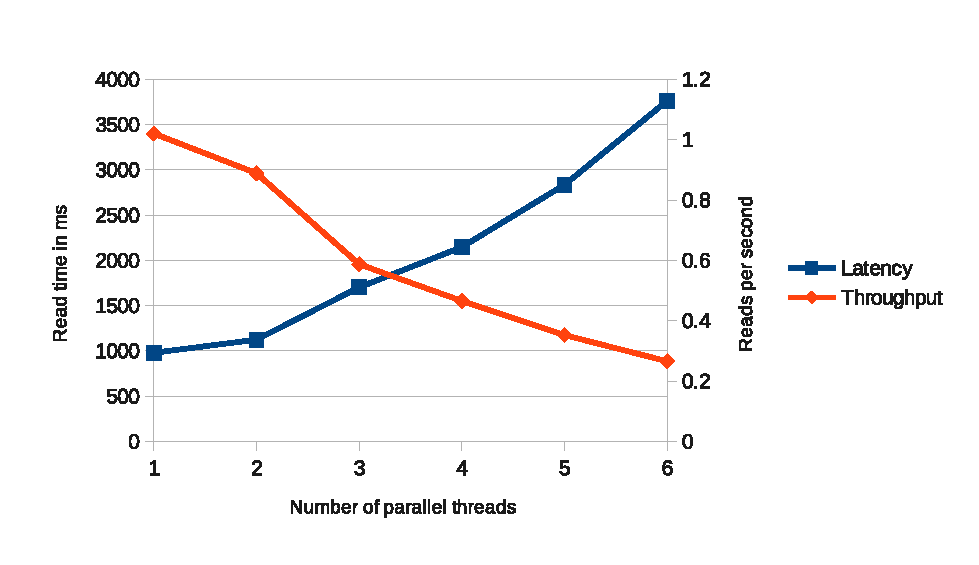
\includegraphics[width=0.8\textwidth]{latencythroughput.eps}\\
  \caption{Plot of service latency and throughput.}
  \label{fig:latecnythroughput}
\end{figure}


\subsection*{Question 7}
\label{sec:pq7} 

The high average of latency seems unjustifiably high. Further analysis of the test results does however give explanations for this. The test data set that represents the Twitter connection graph contains several outliers that have a considerably larger than average amount of connections (e.g. greater than a million entries). This can be explained by publicly interesting Twitter users such as celebrities. The analysis of the experimental results revealed that within the test cases that got ranked very high by the Zipf generator we had 3 such data subsets that where hence queried considerably often. These extremely skewed the distribution of latency times (and therefore throughput). We figure this experimental results are still valid though, as in a real application of our service these subsets could also be queried considerably more often. Figure \ref{fig:cluster} shows the distribution of latency times, and confirms the skew in the distribution. We emphasized the data points that correspond to the large subsets of more than 1 million results ("Greater 1 mio."). One can see that they form a complete separate cluster and the other latency times are much faster.

\begin{figure}
\centering
  \includegraphics[width=0.8\textwidth]{cluster.eps}\\
  \caption{Plot of distribution of latency.}
  \label{fig:cluster}
\end{figure}

We also analysed if miss-hits - that are requests for keys that where not existent - form another cluster. Table \ref{tab:other} reports the test results for latency and throughput, when we separate out the subsets with the large amounts of entries (greater 1 million entries). We show the latency for  the subset of requests where the key was not found ("Key not found"), and all other requests that where found, but do not belong to the set of entries with large result sets ("Other"). The table reviews that the average times do differ between these groups, however the effect is not as significant as for the large data sets.

\begin{table}
\caption{Latency and Throughput without large result subsets.}
\centering
\begin{tabular}{|p{0.2\textwidth}|p{0.2\textwidth}|p{0.2\textwidth}|p{0.2\textwidth}|}
\hline
\multicolumn{2}{|c|}{Key not found} & \multicolumn{2}{|c|}{Other} \\ \hline
Latency (in ms) & Throughput (in reads per second) & Latency (in ms) & Throughput (in reads per second) \\ \hline
17.7839 & 56.2305 & 27.6347 & 36.1864 \\ \hline
17.1237 & 58.3988 & 30.6508 & 32.6255 \\ \hline
17.9104 & 55.8334 & 34.7323 & 28.7917 \\ \hline
15.5843 & 64.1672 & 42.1802 & 23.7078 \\ \hline
10.9129 & 91.6350 & 39.2526 & 25.4760 \\ \hline
18.0697 & 55.3413 & 84.9173 & 11.7762 \\ \hline
\end{tabular}
\label{tab:other}
\end{table}

\subsection*{Question 8}
\label{sec:pq8}
There are a number experiments that we would have liked to do but lacked the necessary time or computing power:

\begin{itemize}
  \item More physical clients: Whenever we used several clients to test our store, we simply created several client threads on a single machine. Since most of our test cases and our main experiment generated considerable workload for the client, we can be certain that the client's hardware limitations have influenced our results. Apart from the limited CPU-power that was available for each client, this also meant that only one request could physically be sent at a time (although, of course, several requests could be sent in short succession). It would have been nice to actually use a much higher number of physical clients to simulate more realistic conditions (maybe with smaller values), and see how this affects latency and throughput. 
  \item Scalability: We ran our store on several machines, none of which had more than four CPU cores. Since one main requirement of the store was concurrency, we could have tested how the store behaves with a much higher number of cores, and if increasing the number of cores actually results in linearly higher throughput (and we therefore have good scalability).
  \item Longterm memory consumption: Although we join adjacent free memory areas wherever possible, our store will probably still suffer from a certain amount of fragmentation when it runs long enough. We could have tracked how much space the store used over time when there are ongoing updates, inserts and deletes.
  \item Behaviour for small values: The performance of our store suffered considerably when huge values (or very long lists of small values) were used, mostly because of the high workload for serialization and deserialization both for the memory mapped file and for transport in the SOAP message. Since SOAP web services in general are a horrible way to access big amounts of data, one would probably use a store like ours for smaller values in practice. We could have made performance tests with test data with much smaller values, which would have allowed us to increase the number of clients and get perhaps more meaningful performance data for any applications that might use such a store in practice.
  \item Concurrency for long-running atomic operations: We did not check the performance of longer operations like atomicScan or bulkPut at all. We could have checked how a bulkPut affects the latency of other parallel operations, we could have compared the performance of bulkPut to that of equivalent insert and update operations, which would be a way to measure the overhead for the RPC invocation, or we could have compared the performance of scan and atomicScan to get an idea how much the locking affects latency.
  \item Performance for real-life access patterns: Our experiment only measured latency for read access. It would be interesting to also check throughput and latency for a realistic mixture of insert, update, read and delete operations.
  \item Impact of wrappers: As stated before, a lot of the store's workload stems from serialization of keys and values. We think that removing ValueImpl entirely (and simply putting strings into ValueListImpl) could have a considerably positive impact on the average latency, especially for lists with many small values. We would have liked to verify this assumption. Since the SOAP envelope is itself a kind of wrapper and SOAP is not known for its great performance, it would also have been interesting to check how a more lightweight protocol like a RESTful service would influence latency.
  
\end{itemize}

\subsection*{Question 9}
\label{sec:pq9}
Our implementation of \texttt{atomicScan} differs from the normal \texttt{scan} only in one way. At the start of the function, we first acquire a read lock on the key-to-space-map, then we get read locks for all keys that are currently in the map. We do this in order, from the smallest key to the largest, in order to avoid deadlocks. Once we have all the locks, we execute the scan, i.e. we iterate through all keys, check if they are in the specified range, and return a list of those that are. The evaluation of the predicate is implemented in KeyValueBaseImpl (as opposed to the rest, which is in IndexImpl) and is identical to that of regular scan. Finally, we release the locks on all the keys and subsequently the lock on the map.

For \texttt{bulkPut}, our approach is a little different. Here we know beforehand which values we will manipulate, which is why we only need to lock the keys belonging to these values. Since we were specifically asked to ensure that all users see the store either in its state before the bulkPut or in the state after its completion, i.e. no in-between-states are visible, we get write locks on all those keys at the beginning of the method and only release them when all the work is done. This is the same approach we used in atomicScan, but here it is actually necessary to ensure the intended behaviour, whereas for atomicScan it was only the most convenient of many possible solutions, because it guarantees that there are no deadlocks or cascading aborts. As usual when we request several locks at once, we do so in the intrinsic order of their respective keys, which is possible because keys are comparable. We do not have to lock our key-to-space-map for the main procedure, since we do not care if new keys and values are concurrently inserted into the map as long as they do not conflict with the keys we are working on. For the actual work, i.e. inserting and updating values, we use the respective functions we implemented before.
 
\begin{thebibliography}{1}

\bibitem[Schroeder2007]{Schroeder2007} Bianca Schroeder and Garth A. Gibson. 2007. Disk failures in the real world: what does an MTTF of 1,000,000 hours mean to you?. In Proceedings of the 5th USENIX conference on File and Storage Technologies Schroeder2007(FAST '07). USENIX Association, Berkeley, CA, USA, , Article 1 .

\bibitem[Dean]{Dean} Jeff Dean. n.y. as found in: Marcos Vaz Salles. PCSD. lecture: Experimental Design - Concurrency Control: 2PL, p.9.

\bibitem[Gray1994]{Gray1994} Gray et al.: Quickly Generating Billion-Record Synthetic Databases. SIGMOD 1994: 243 - 252. Tech report available at: \url{http://research.microsoft.com/~gray/papers/SyntheticDataGen.doc}.

\end{thebibliography}



\end{document}
